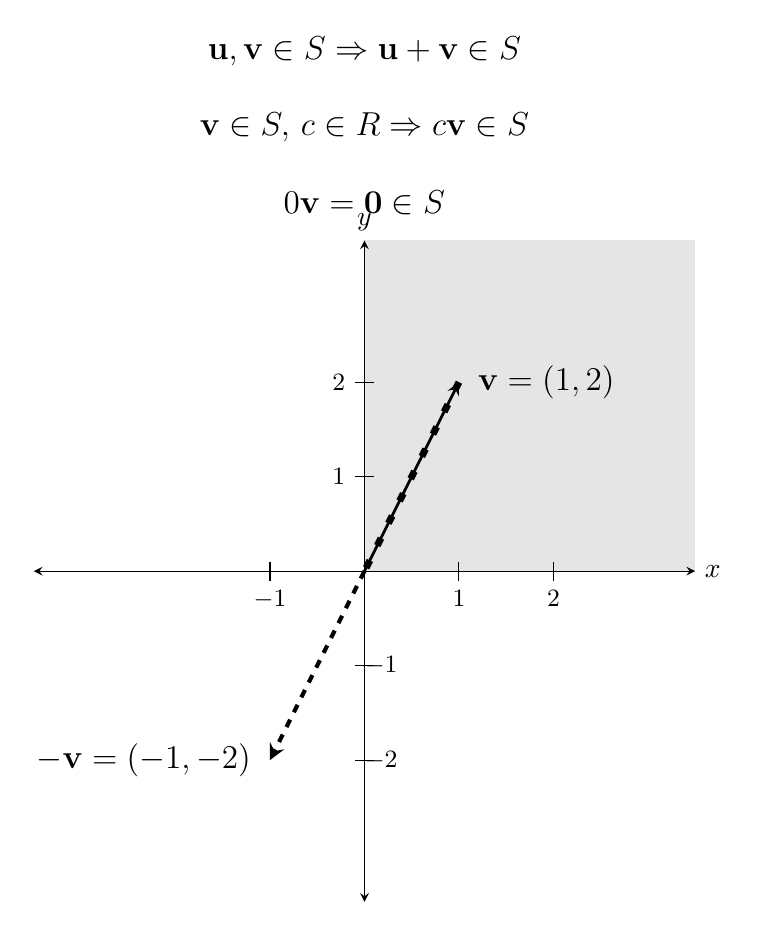
\begin{tikzpicture}[x=1.2cm, y=1.2cm]

    \gid{formula-addition-closure}{
        \node[font=\large] at (0, 4.5) {$\mathbf{u}, \mathbf{v} \in S \Rightarrow \mathbf{u} + \mathbf{v} \in S$};
    }
    
    \gid{formula-scalar-closure}{
        \node[font=\large] at (0, 3.7) {$\mathbf{v} \in S, \, c \in \mathbb{R} \Rightarrow c\mathbf{v} \in S$};
    }
    
    \gid{formula-zero-requirement}{
        \node[font=\large] at (0, 2.9) {$0\mathbf{v} = \mathbf{0} \in S$};
    }
    
    \begin{scope}[shift={(0,-1)}]
        \gid{first-quadrant-region}{
            \fill[black, opacity=0.1] (0, 0) rectangle (3.5, 3.5);
        }
        
        \gid{axes}{
            \draw[<->, >=stealth] (-3.5, 0) -- (3.5, 0) node[right] {$x$};
            \draw[<->, >=stealth] (0, -3.5) -- (0, 3.5) node[above] {$y$};
            
            \draw (-1, 0.1) -- (-1, -0.1) node[below] {\small $-1$};
            \draw (1, 0.1) -- (1, -0.1) node[below] {\small $1$};
            \draw (2, 0.1) -- (2, -0.1) node[below] {\small $2$};
            \draw (0.1, 1) -- (-0.1, 1) node[left] {\small $1$};
            \draw (0.1, 2) -- (-0.1, 2) node[left] {\small $2$};
            \draw (0.1, -1) -- (-0.1, -1) node[right] {\small $-1$};
            \draw (0.1, -2) -- (-0.1, -2) node[right] {\small $-2$};
        }
        
        \gid{vector-v}{
            \draw[->, >=stealth, line width=1.0pt] (0,0) -- (1,2);
        }
        
        \gid{backward-extension}{
            \draw[loosely dashed, line width=2.5pt] (1,2) -- (0,0);
        }
        
        \gid{negative-vector}{
            \draw[->, >=stealth, dashed, line width=1.5pt] (0,0) -- (-1,-2);
        }
        
        \gid{label-v}{
            \node[right] at (1.1, 2) {\large $\mathbf{v}=(1,2)$};
        }
        
        \gid{label-negative-v}{
            \node[left] at (-1.1, -2) {\large $-\mathbf{v}=(-1,-2)$};
        }
    \end{scope}
\end{tikzpicture}